% section
\section{Related work} \label{section::related}
 This section will describe a range of state-of-the-art architectures for \glqq unsupervised\grqq image-/video-prediction. Image-/video-prediction is a very broad 
 field, but almost all (investigated by me) state-of-the-art solutions
 for image-/video-prediction share one common part, the recurrent module. LSTM's are the most used modules in image-/video-prediction, as they are able to store information over a long period of time, despite
 the standard RNN (recurrent neural network). All algorithms described here have a different way to perform image prediction, but all use a type of LSTM to store the time-series information.
 \\\\
 It is very common for this type of papers, that the authors start their experiments by using a synthetic dataset. In the most cases this is MovingMNIST \cite{LeCun1998} and then afterwards performing
 tests on natural images. For natural images, the authors often use action-recognition datasets, because the camera is fixed and only objects/people in the scenery are moving. Another approach
 is using natural image datasets, where the camera is also moving through the scenery (egocentric movement), for example Kitti dataset \cite{Geiger2013}.
 This dataset consists of natural images from different car drives through the city and residential area of Karlsruhe in Germany.
 In this dataset not only objects in the scenery are moving, but also the camera has a self-motion, which can be very tricky for image prediction algorithms to 
 \glqq understand\grqq.
 
 % subsection
 \subsection{LSTM Autoencoder} \label{subsection::lstm_autoencoder}
  The paper \glqq Unsupervised Learning of Video Representations using LSTMs\grqq by Srivastava et al. \cite{Srivastava2015} is using a LSTM~\ref{subsection::lstm} from Graves 
  \cite{Graves2013} in an autoencoder architecture~\ref{subsection::autoencoder} for image reconstruction and future image prediction.
  The architecture for image reconstruction and image prediction is the same, the necessary behavior is achieved only through the different training.
  For image reconstruction, the network will get the already seen image sequence to compare and compute the error for. For image prediction, the network gets
  the next $n$ frames, which it predicts to compare and compute the error for.
  Another use-case given by the authors is a composed model, in which image reconstruction and image prediction is done simultaneously. Therefore they have
  one encoder and two different decoder, one decoder for image reconstruction and one for image prediction.
  This is an example of how representation learning algorithms (neural networks) are able to learn different behavior, due to the error computation and following
  backpropagation.
  The architecture is often used as a baseline in newer and more advanced architectures, because it consists of the standard LSTM as recurrent module.
  \\\\
  Due to the fact, that the LSTM module is not able to handle multi-dimensional data as is, the images need to be reshaped at the input and also at the output again. The authors use
  MovingMNIST \cite{LeCun1998} as synthetic dataset, where every image is of size $(64 \times 64 \times 1)$. Therefore the image is vectorized into $(64 \cdot 64 \times 1)$ $=$ $(4096 \times 1)$.
  This MovingMNIST implementation consists of two digits inside every frame. The authors input $10$ images and output the next $10$ images, therefore they perform 
  multi-frame prediction.
  \\\\
  The model is end-to-end differentiable and trained using BPTT.
  For the synthetic dataset, the model is trained using cross-entropy loss with logits (which is just the cross-entropy loss followed by a sigmoid function), for 
  natural image datasets using MSE (mean-squared error) \cite{Zhao2017}.
  \begin{figure}[H]
   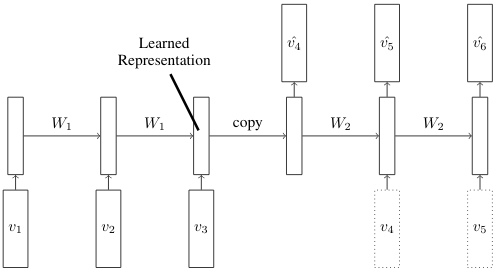
\includegraphics[width=0.45\textwidth]{../Images/srivastava.png}
   \centering
   \caption{Architecture for future image prediction \cite{Srivastava2015}}
   \label{fig:lstm_architecture}
  \end{figure}
  \begin{figure}[H]
   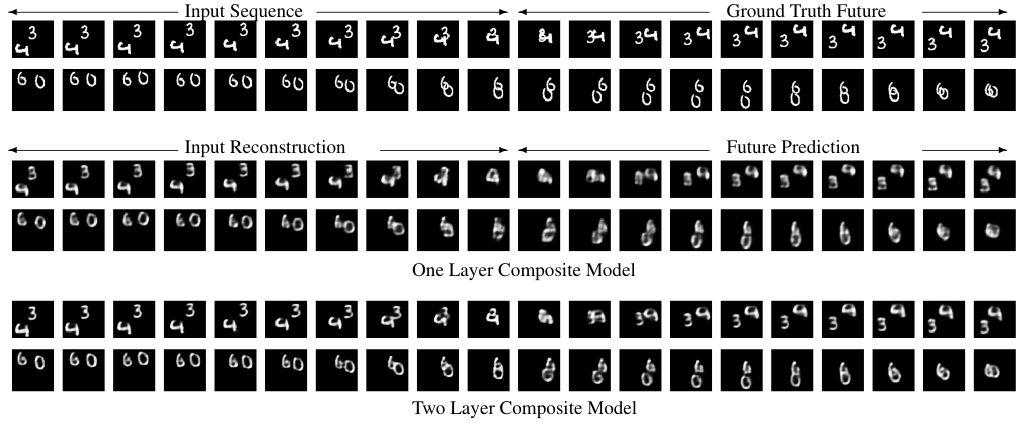
\includegraphics[width=0.85\textwidth]{../Images/srivastava_results_mnist.png}
   \centering
   \caption{Results for MovingMNIST \cite{Srivastava2015}}
   \label{fig:lstm_results}
  \end{figure}

 % subsection
 \subsection{ConvLSTM Autoencoder} \label{subsection::convlstm_autoencoder}
  The paper \glqq Convolutional LSTM Network: A Machine Learning Approach for Precipitation Nowcasting\grqq by Shi et al. \citep{Shi2015} is using a similar 
  architecture as Srivastava et al. in
  figure~\ref{fig:lstm_architecture}, but instead of using the standard LSTM, they use a novel ConvLSTM~\ref{subsection::convlstm}. The ConvLSTM used in this 
  architecture is with peephole connection~\ref{subsection::convlstm}.
  \\\\
  This architecture outperforms the implementation of Srivastava et al., because it \glqq captures spatiotemporal correlations better\grqq.
  This model is, same as LSTM Autoencoder~\ref{subsection::lstm_autoencoder} end-to-end differentiable and trained using BPTT. It also uses the cross-entropy loss with logits for the synthetic dataset 
  (MovingMNIST) experiment. In this MovingMNIST implementation, every frame consists of three digits. As in the architecture above, the authors here input $10$ images and output $10$. This architecture is only used for forecasting by the authors, but due to the architecture choice could be also useful for image
  reconstruction. This architecture is used as one of the baselines for the performed experiments in section~\ref{section::experiments}.
  \begin{figure}[H]
   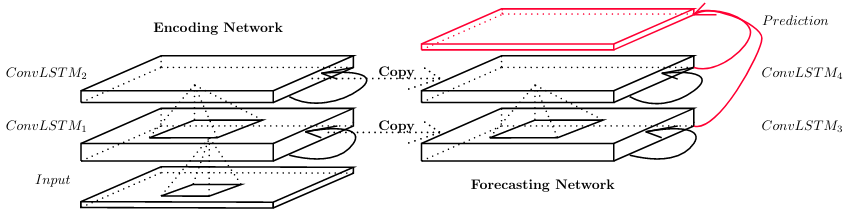
\includegraphics[width=0.7\textwidth]{../Images/shi.png}
   \centering
   \caption{Future image prediction model \cite{Shi2015}}
   \label{fig:convlstm_architecture}
  \end{figure}
  \begin{figure}[H]
   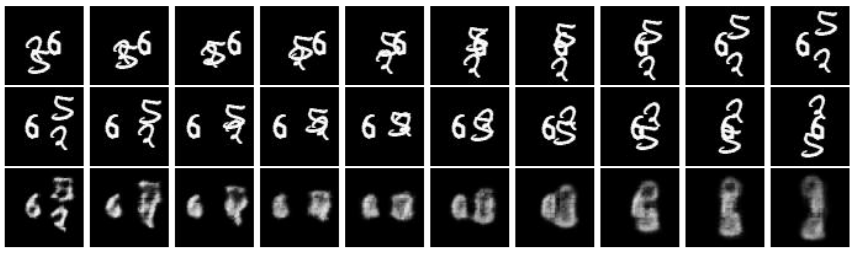
\includegraphics[width=0.5\textwidth]{../Images/shi_results_mnist.png}
   \centering
   \caption{Results for MovingMNIST. \textbf{First Row:} 10 input images, \textbf{Second Row:} Ground truth next images, \textbf{Third Row:} Prediction of 3-layer implementation \cite{Shi2015}}
   \label{fig:convlstm_results}
  \end{figure}
 
 % subsection
 \subsection{Spatio-temporal Video Autoencoder}
  The paper \glqq Spatio-temporal Video Autoencoder With Differentiable Memory\grqq by Patraucean et al. \cite{Patraucean2015} describes a more complex architecture, in which the authors
  nest a temporal autoencoder inside a spatial autoencoder.
  \\\\  
  The spatial autoencoder is a simple undercomplete autoencoder~\ref{subsection::autoencoder}, where the decoder uses nearest-neighbor
  upsampling to get the output image size correct. The temporal autoencoder consists of a ConvLSTM (without peephole), which works as the temporal 
  encoder and an optical flow convolutional module, which works
  as the temporal decoder.
  \\\\
  The network idea is to insert the image sequence $X$, which will create an optical flow map. This optical flow map is then applied on the last given image, to 
  shift every pixel to it's new position. This will create the next image. The idea behind this is given in \glqq Spatial Transformer Networks\grqq by Jadeberg et 
  al. \cite{Jadeberg2015}, where they invent an image sampler to apply a projective transformation on an image to e.g. rotate and rescale it. Despite the initial 
  idea
  of Jadeberg et al., the authors here use the image sampler with the optical flow map, which can be seen as a projective transformation, but different for every 
  pixel, instead of having one transformation for the whole image.
  \\\\
  The model is end-to-end differentiable and trained using BPTT. The authors also used MovingMNIST as synthetic dataset and use the cross-entropy loss with logits as reconstruction error for it. The 
  MovingMNIST implementation is the same as in LSTM Autoencoder~\ref{subsection::lstm_autoencoder} (With two digits per frame.).
  \\\\
  In contrast to the other two algorithms, this architecture is only capable of doing one-frame prediction as is. The authors input $19$ images and output one 
  image. It is possible to have multi-frame prediction, by e.g. adding a feedback loop, in which the output of the network is used as the next frame in the input 
  sequence. Therefore the network should be also trained for one-frame prediction and then simply used for multi-frame prediction. The architecture is also used
  as one of the baselines in the experiments~\ref{section::experiments}.
  \begin{figure}[H]
   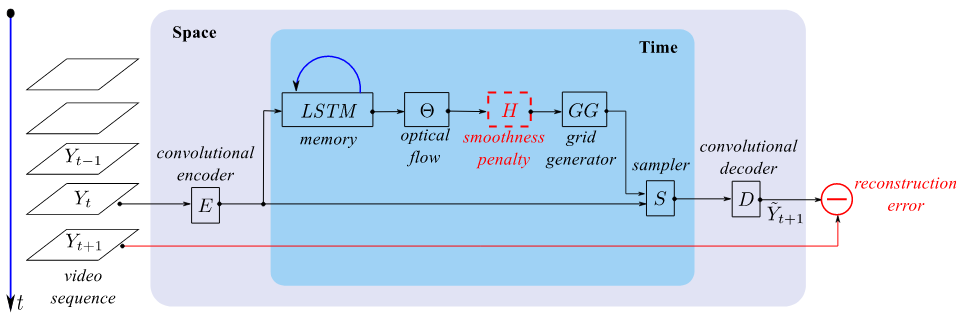
\includegraphics[width=0.7\textwidth]{../Images/patraucean.png}
   \centering
   \caption{Spatio-temporal Video Autoencoder \cite{Patraucean2015}}
   \label{fig:spatiotemp_architecture}
  \end{figure}
  \begin{figure}[H]
   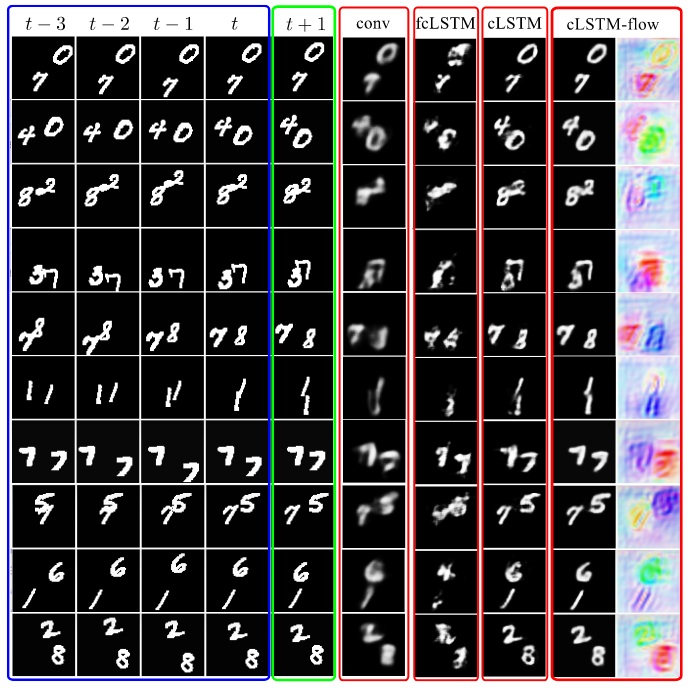
\includegraphics[width=0.45\textwidth]{../Images/patraucean_results_mnist.png}
   \centering
   \caption{Results for MovingMNIST. \textbf{conv:} Is a simple convolutional autoencoder, without recurrent module, \textbf{fcLSTM:} LSTM Autoencoder~\ref{subsection::lstm_autoencoder},
   \textbf{cLSTM:} ConvLSTM Autoencoder~\ref{subsection::convlstm_autoencoder}, \textbf{cLSTM-flow:} Spatio-temporal Video Autoencoder with extra output of flow-map. \cite{Patraucean2015}}
   \label{fig:spatiotemp_results}
  \end{figure}
 
 % subsection
 \subsection{PredNet}
  The paper \glqq Deep Predictive Coding Networks For Video Prediction And Unsupervised Learning\grqq by Lotter et al. \cite{Lotter2016} composes an architecture, which is informally named
  \textbf{PredNet}. It describes a network architecture based on the concept of \glqq predictive coding\grqq \cite{Rao1999}, \cite{Friston2005}. It is also one of the baselines for the experiments performed
  in section~\ref{section::experiments}.
  \\\\  
  The network consists of an arbitrary amount of layers, the amount of layers (depth of the network) can be treated as a hyperparameter. Every layer consists
  of an input module $A{_l}^t$, prediction module $\hat{A{_l}^t}$, representation module $R{_l}^t$ and error module $E{_l}^t$.\\
  $l$ is the corresponding layer, $t$ the timestamp.
  \begin{figure}[H]
   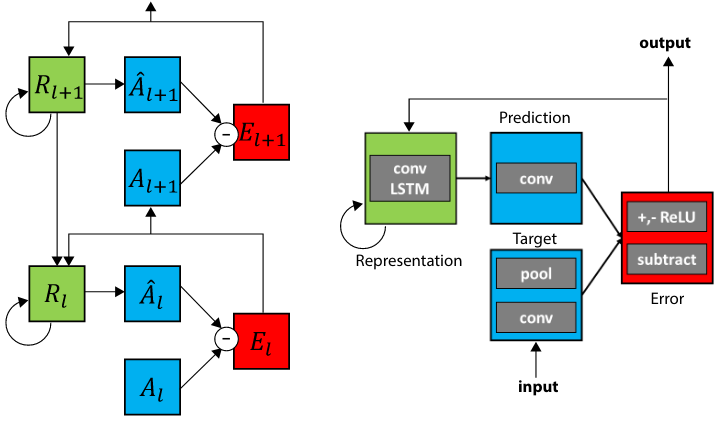
\includegraphics[width=0.55\textwidth]{../Images/lotter.png}
   \centering
   \caption{\textbf{Left:} PredNet architecture with two layers, \textbf{Right:} \glqq Module operations for case of video sequences\grqq \cite{Lotter2016}}
   \label{fig:lotter_architecture}
  \end{figure}
  \begin{equation}
   A{_l}^t = \begin{cases} x_t & l = 0 \\ MaxPool(ReLU(Conv(E_{l-1}^t))) & l > 0 \end{cases}
  \end{equation}
  \begin{equation}
   \hat{A_l^t} = ReLU(Conv(R_l^t)
  \end{equation}
  \begin{equation}
   E_l^t = [ReLU(\hat{A_l^t} - A_l^t); ReLU(A_l^t - \hat{A_l^t})]
  \end{equation}
  \begin{equation}
   R_l^t = ConvLSTM(E_l^{t-1}, R_l^{t-1}, Upsample(R_{l+1}^t)
  \end{equation}\noindent
 Despite the other algorithms, this architecture is doing the prediction in every step the network does. The typical way (at least for the already described 
 algorithms), is to insert the full input sequence and after computing through the whole sequence outputting the predicted next frame. This architecture will go
 through every image of the sequence, but for every input of the input sequence, the network already outputs the predicted next frame. This can be seen in the
 predicted images, because the first predicted image doesn't have any information about the sequence at all, but is just randomly distributed in some
 kind of gray-scale.
 \\\\
 Another very important difference, is that the network is not using a type of reconstruction error as the networks above do. Here they compose the model to
 have different output modes. One is for error computation, the other for prediction. During the error computation, the network uses a loss function, which takes
 the given amount of layer and time into account. Regarding the authors, this is done, same as in Predictive Coding.
 \begin{equation}
  L_t = \sum_{t}\lambda_t \sum_l \frac{\lambda_l}{n_l} \sum_{n_l}E_l^t
 \end{equation}
 The authors decided to use a different synthetic dataset. They used a self created dataset with rotating faces, created with \href{https://facegen.com/}
 {FaceGen}.
 \begin{figure}[H]
   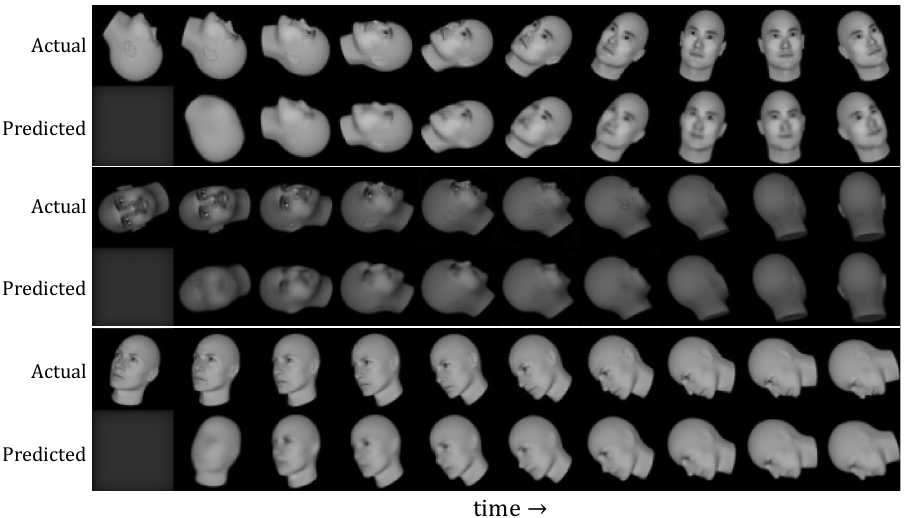
\includegraphics[width=0.65\textwidth]{../Images/prednet.png}
   \centering
   \caption{Results for the rotating faces dataset \cite{Lotter2016}.}
   \label{fig:lotter_rotation}
 \end{figure}\noindent
 Elsayed et al. \cite{Elsayed2018} added a novel LSTM architecture to PredNet and performed synthetic tests on the standard PredNet implementation
 using MovingMNIST.
 \begin{figure}[H]
   \centering
   \subfloat[Ground truth]{{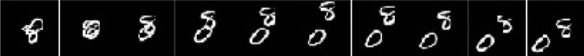
\includegraphics[width=0.55\textwidth]{../Images/prednet_mnist_actual.png} }} 
   \qquad
   \subfloat[ConvLSTM]{{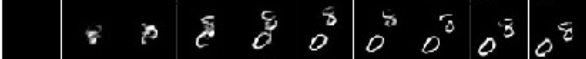
\includegraphics[width=0.55\textwidth]{../Images/prednet_mnist_prediction.png} }} 
   \caption{Results for MovingMNIST \cite{Elsayed2018}.}
   \label{figure::elsayed_mnist}
  \end{figure}\noindent
 
 % subsection
 \subsection{PredRNN} \label{subsection::PredRNN}
  The paper \glqq PredRNN: Recurrent Neural Networks for Predictive Learning using Spatiotemporal LSTMs\grqq by Wang et al. \cite{Wang2017} describes a novel
  LSTM module, named Spatiotemporal LSTM (ST-LSTM) and an architecture build from this sub-module named PredRNN.
  This ST-LSTM consists of the typical temporal memory, but extends this by having an additional spatiotemporal memory.
  \begin{equation}
   g_t = tanh(W_{xg} \ast X_t + W_{hg} \ast H_{t-1}^l + b_g)
  \end{equation}
  \begin{equation}
   i_t = \sigma(W_{xi} \ast X_t + W_{hi} \ast H_{t-1}^l +b_i)
  \end{equation}
  \begin{equation}
   f_t = \sigma(W_{xf} \ast X_t + W_{hf} \ast H_{t-1}^l + b_f)
  \end{equation}
  \begin{equation}
   C_t^l = f_t \odot C_{t-1}^l + i_t \odot g_t
  \end{equation}
  \begin{equation}
   g_t\prime = tanh(W_{xg}\prime \ast X_t + W_{mg} \ast M_t^{l-1} + b_g\prime)
  \end{equation}
  \begin{equation}
   i_t\prime = \sigma(W_{xi}\prime \ast X_t + W_{mi} \ast M_t^{l-1} + b_i\prime)
  \end{equation}
  \begin{equation}
   f_t\prime = \sigma(W_{xf}\prime \ast X_t + W_{mf} \ast M_t^{l-1} + b_f\prime)
  \end{equation}
  \begin{equation}
   M_t^l = f_t\prime \odot M_t^{l-1} + i_t\prime \odot g_t\prime
  \end{equation}
  \begin{equation}
   o_t = \sigma(W_{xo} \ast X_t + W_{ho} \ast H_{t-1}^l + W_{co} \ast C_t^l + W_{mo} \ast M_t^l + b_o)
  \end{equation}
  \begin{equation}
   H_t^l = o_t \odot tanh(W_{1 \times 1} \ast [C_t^l, M_t^l])
  \end{equation}
  \begin{figure}[H]
   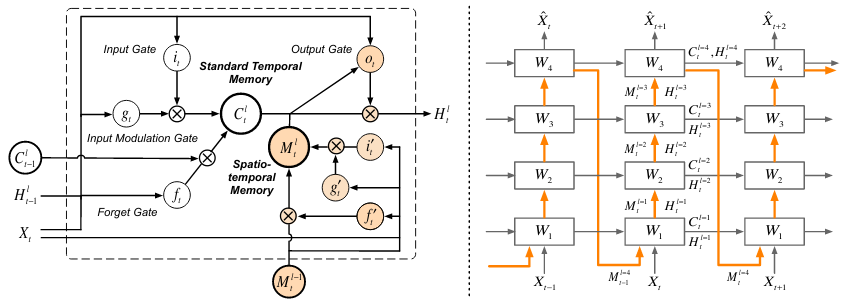
\includegraphics[width=0.8\textwidth]{../Images/wang.png}
   \centering
   \caption{\textbf{Left:} ST-LSTM architecture, \textbf{Right:} PredRNN architecture \cite{Wang2017}}
   \label{fig:wang_architecture}
  \end{figure}\noindent
  The model is end-to-end differentiable and trained using BPTT. The authors use MovingMNIST as synthetic dataset, with 20 images per sequence, where ten images
  are used as input and the other ten as output. They also use two digits per frame with an image size of $(64 \times 64 \times 1)$.
  This architecture is the baseline, which replaces the ConvLSTM's in the previous architectures, in the experiments~\ref{section::experiments}.
  \begin{figure}[H]
   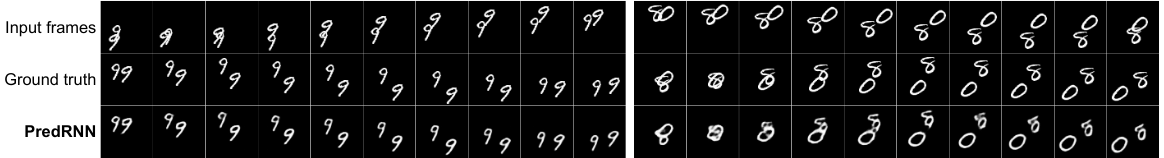
\includegraphics[width=1.0\textwidth]{../Images/predrnn_mnist.png}
   \centering
   \caption{Results for MovingMNIST \cite{Wang2017}.}
   \label{fig:predrnn_mnist}
  \end{figure}\noindent
\\\\
All of the seen algorithms in this section have different approaches or ideas to get to a similar result.
Srivastava et al. \cite{Srivastava2015} start, by leveraging the LSTM in an Autoencoder architecture to achieve state-of-the-art image-/video-prediction.
Shi et al. \cite{Shi2015} then invent a ConvLSTM module, which is placed in the previous Autoencoder architecture to achieve state-of-the-art performance.
Patraucean et al. \cite{Patraucean2015} then leverage optical flow as a new approach for image-/video-prediction and also start splitting information in space and time, but also stick to a ConvLSTM module as recurrent module and the overall Autoencoder architecture.
Lotter et al. \cite{Lotter2016} introduce the neuro-scientific topic of
predictive coding to image-/video-prediction, which also uses a ConvLSTM module as recurrent module but isn't an Autoencoder architecture.
Wang et al. \cite{Wang2017} invent a novel LSTM module, named ST-LSTM and also the novel state-of-the-art image-/video-prediction architecture named PredRNN, in
which they implement their newly invented ST-LSTM module.
\\\\
It emerges from the seen papers, that all of the approaches share
the idea of using a recurrent module, the LSTM and many of them also use the Autoencoder architecture to perform state-of-the-art image-/video-prediction.